\documentclass{standalone}
\usepackage{tikz, xcolor}
\usetikzlibrary{shapes,arrows}

\begin{document}

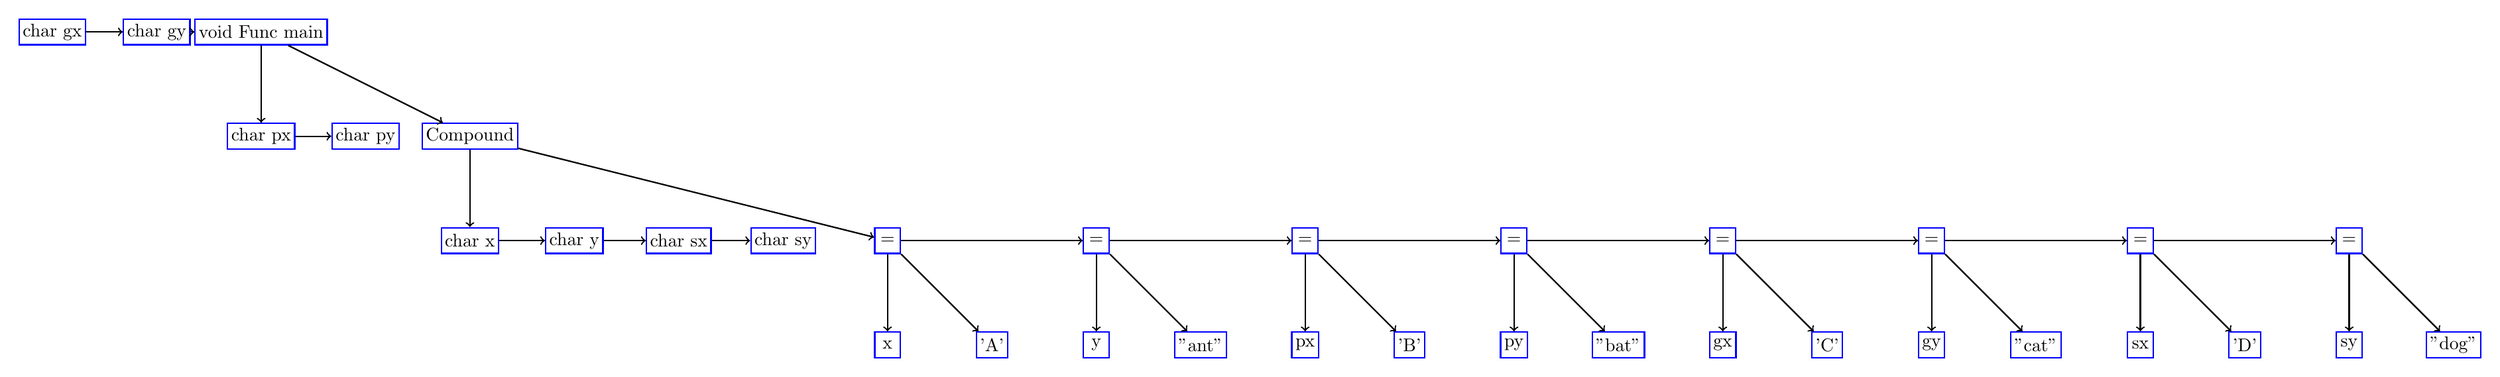
\begin{tikzpicture}[thick, scale=2.0]
\tikzstyle{vertexr}=[rectangle, draw=blue, thick, minimum size=14pt, inner sep=2pt]
\tikzstyle{vertexc}=[circle, draw=blue, thick, inner sep=2pt]
\tikzstyle{drawstyle}=[thick, ->]

\node[vertexr] (G0x0) at (0,0) {char gx};
\node[vertexr] (G1x0) at (1,0) {char gy};
\node[vertexr] (G2x0) at (2,0) {void Func main};
\node[vertexr] (G2x1) at (2,-1) {char px};
\node[vertexr] (G3x1) at (3,-1) {char py};
\draw[drawstyle] (G2x1) -- (G3x1);
\draw[drawstyle] (G2x0) -- (G2x1);
\node[vertexr] (G4x1) at (4,-1) {Compound};
\node[vertexr] (G4x2) at (4,-2) {char x};
\node[vertexr] (G5x2) at (5,-2) {char y};
\node[vertexr] (G6x2) at (6,-2) {char sx};
\node[vertexr] (G7x2) at (7,-2) {char sy};
\draw[drawstyle] (G6x2) -- (G7x2);
\draw[drawstyle] (G5x2) -- (G6x2);
\draw[drawstyle] (G4x2) -- (G5x2);
\draw[drawstyle] (G4x1) -- (G4x2);
\node[vertexr] (G8x2) at (8,-2) {=};
\node[vertexr] (G8x3) at (8,-3) {x};
\draw[drawstyle] (G8x2) -- (G8x3);
\node[vertexr] (G9x3) at (9,-3) {'A'};
\draw[drawstyle] (G8x2) -- (G9x3);
\node[vertexr] (G10x2) at (10,-2) {=};
\node[vertexr] (G10x3) at (10,-3) {y};
\draw[drawstyle] (G10x2) -- (G10x3);
\node[vertexr] (G11x3) at (11,-3) {"ant"};
\draw[drawstyle] (G10x2) -- (G11x3);
\node[vertexr] (G12x2) at (12,-2) {=};
\node[vertexr] (G12x3) at (12,-3) {px};
\draw[drawstyle] (G12x2) -- (G12x3);
\node[vertexr] (G13x3) at (13,-3) {'B'};
\draw[drawstyle] (G12x2) -- (G13x3);
\node[vertexr] (G14x2) at (14,-2) {=};
\node[vertexr] (G14x3) at (14,-3) {py};
\draw[drawstyle] (G14x2) -- (G14x3);
\node[vertexr] (G15x3) at (15,-3) {"bat"};
\draw[drawstyle] (G14x2) -- (G15x3);
\node[vertexr] (G16x2) at (16,-2) {=};
\node[vertexr] (G16x3) at (16,-3) {gx};
\draw[drawstyle] (G16x2) -- (G16x3);
\node[vertexr] (G17x3) at (17,-3) {'C'};
\draw[drawstyle] (G16x2) -- (G17x3);
\node[vertexr] (G18x2) at (18,-2) {=};
\node[vertexr] (G18x3) at (18,-3) {gy};
\draw[drawstyle] (G18x2) -- (G18x3);
\node[vertexr] (G19x3) at (19,-3) {"cat"};
\draw[drawstyle] (G18x2) -- (G19x3);
\node[vertexr] (G20x2) at (20,-2) {=};
\node[vertexr] (G20x3) at (20,-3) {sx};
\draw[drawstyle] (G20x2) -- (G20x3);
\node[vertexr] (G21x3) at (21,-3) {'D'};
\draw[drawstyle] (G20x2) -- (G21x3);
\node[vertexr] (G22x2) at (22,-2) {=};
\node[vertexr] (G22x3) at (22,-3) {sy};
\draw[drawstyle] (G22x2) -- (G22x3);
\node[vertexr] (G23x3) at (23,-3) {"dog"};
\draw[drawstyle] (G22x2) -- (G23x3);
\draw[drawstyle] (G20x2) -- (G22x2);
\draw[drawstyle] (G18x2) -- (G20x2);
\draw[drawstyle] (G16x2) -- (G18x2);
\draw[drawstyle] (G14x2) -- (G16x2);
\draw[drawstyle] (G12x2) -- (G14x2);
\draw[drawstyle] (G10x2) -- (G12x2);
\draw[drawstyle] (G8x2) -- (G10x2);
\draw[drawstyle] (G4x1) -- (G8x2);
\draw[drawstyle] (G2x0) -- (G4x1);
\draw[drawstyle] (G1x0) -- (G2x0);
\draw[drawstyle] (G0x0) -- (G1x0);
\end{tikzpicture}
\end{document}
Number of warnings: 0
Number of errors: 0
